\documentclass[14pt]{beamer}


\usepackage{color}
\usepackage{tikz}


\mode<presentation>
{
\usetheme{AlpesLasers}
\setbeamercovered{transparent}
  %\setbeamertemplate{footline}[frame number] 
  %\setbeamertemplate{navigation symbols}{ 
  %\hskip 0.3cm
  %\insertframenumber / \inserttotalframenumber  % <<< frame #
  %\insertpagenumber / \insertpresentationendpage % <<< page #
%} 
}

% font definitions, try \usepackage{ae} instead of the following
% three lines if you don't like this look
\usepackage{listings}
\lstloadlanguages{python}

\usepackage{mathptmx}
\usepackage[scaled=.90]{helvet}
\usepackage{courier}
\usepackage[T1]{fontenc}
\usepackage[english]{babel}
\usepackage[latin1]{inputenc}
\title{Why PYTHON is THE computer language for physicists}
\subtitle{A little overview}
\author{St\'ephane Poss}
\date{\today}
% This is only inserted into the PDF information catalog. Can be left
% out.
\subject{PYTHON}

\lstdefinestyle{custompy}{
  belowcaptionskip=1\baselineskip,
  breaklines=true,
  xleftmargin=\parindent,
  language=python,
  showstringspaces=false,
  basicstyle=\footnotesize\ttfamily,
  keywordstyle=\bfseries\color{green!40!black},
  commentstyle=\itshape\color{purple!40!black},
  identifierstyle=\color{blue},
  stringstyle=\color{orange},
}
\lstdefinestyle{customsh}{
  belowcaptionskip=1\baselineskip,
  breaklines=true,
  xleftmargin=\parindent,
  language=bash,
  showstringspaces=false,
  basicstyle=\footnotesize\ttfamily,
  keywordstyle=\bfseries\color{green!40!black},
  commentstyle=\itshape\color{purple!40!black},
  identifierstyle=\color{blue},
  stringstyle=\color{orange},
}
\lstdefinestyle{customcpp}{
  belowcaptionskip=1\baselineskip,
  breaklines=true,
  xleftmargin=\parindent,
  language=C++,
  showstringspaces=false,
  basicstyle=\footnotesize\ttfamily,
  keywordstyle=\bfseries\color{green!40!black},
  commentstyle=\itshape\color{purple!40!black},
  identifierstyle=\color{blue},
  stringstyle=\color{orange},
}

\begin{document}
\begin{frame}[plain]
\titlepage
\end{frame}

\begin{frame}
\tableofcontents
\end{frame}

\section{What is PYTHON?}

\begin{frame}
\frametitle{Origins of the language}
\begin{columns}
\column{0.59\textwidth}
Guido Van Rossum:
\begin{itemize}
\item Dutch
\item Computer scientist
\item Benevolent Dictator For Life
\end{itemize}
~\\
1989: first version coded during Christmas break
\column{0.4\textwidth}
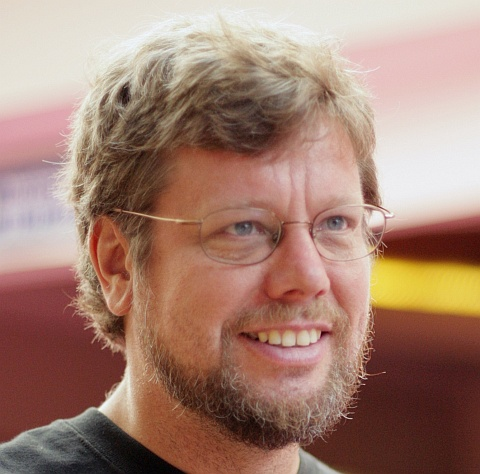
\includegraphics[width=\textwidth]{guido.jpg}\\

\includegraphics[width=4cm]{PythonProgLogo.png}
\end{columns}
\end{frame}

\begin{frame}
\frametitle{Current status}

\includegraphics[width=\textwidth]{python-logo-master-v3-TM.png}

\begin{itemize}
\item Open Source, free
\item 2.7: since 2010, still supported
\item 3.4: since 2014, fixed some of the language flaws. Recommended.
\end{itemize}
\end{frame}

\section{Why use it?}

\begin{frame}
\frametitle{Scripting language}

\lstinputlisting[style=customsh]{intro.py}

\begin{itemize}
\item Much better than Perl/Bourne again shell (bash)/Javascript
\item No compilation needed
\item Easy to test code bits
\end{itemize}
\end{frame}

\begin{frame}
\frametitle{Object Oriented language}
\begin{center}
\alert{Everything is an object!}
\end{center}
\lstinputlisting[style=custompy]{oo.py}
\end{frame}

\begin{frame}
\frametitle{Duck typing}
\begin{quote}
When I see a bird that walks like a duck and swims like a duck and quacks like a duck, I call that bird a duck.\footnote{ Heim, Michael (2007). Exploring Indiana Highways. Exploring America's Highway. p. 68. ISBN 978-0-9744358-3-1.}
\end{quote}
\end{frame}

\begin{frame}
\frametitle{Duck typing II}
Python is:
\begin{itemize}
\item strongly typed
\lstinputlisting[style=custompy]{strongtype.py}
\item not statically typed
\lstinputlisting[style=custompy]{statictype.py}
\end{itemize}
\end{frame}

\begin{frame}
\frametitle{Easy to read}
'Natural' language:
\lstinputlisting[style=custompy]{natural.py}
\end{frame}

\begin{frame}
\frametitle{Easy to read (II)}
Concise:
\lstinputlisting[style=custompy]{concise.py}
\end{frame}

\begin{frame}
\frametitle{Easy to read (III)}
Easy iteration:
\lstinputlisting[style=custompy]{iterator.py}
\end{frame}

\begin{frame}
\frametitle{Easy to read (IV)}
Dictionaries:
\lstinputlisting[style=custompy]{dict.py}
Can contain anything. Keys must be unmutable.
\end{frame}

\begin{frame}
\frametitle{Easy to read: example}
\lstinputlisting[style=custompy]{prime.py}
\end{frame}

\begin{frame}
\frametitle{Easy to write}
Typical C++ construct:
\lstinputlisting[style=customcpp]{map.cpp}
~\\
Equivalent PYTHON code:
\lstinputlisting[style=custompy]{map.py}
Python dictionaries replace most C/C++ structures
\end{frame}

\begin{frame}
\frametitle{Easy to write (II)}
C++ construct:
\lstinputlisting[style=customcpp]{cppcomp.cpp}
PYTHON:
\lstinputlisting[style=custompy]{pycomp.py}
\end{frame}

\begin{frame}
\frametitle{Class definitions}
C++ (in .h):
\lstinputlisting[style=customcpp]{class.h}
in .cpp:
\lstinputlisting[style=customcpp]{imp.cpp}
\end{frame}

\begin{frame}
\frametitle{Class definitions}
PYTHON:
\lstinputlisting[style=custompy]{class.py}
\end{frame}


\begin{frame}
\frametitle{Multiple inheritance}
\lstinputlisting[style=custompy]{inheritance.py}

No 'Diamond of doom' problems!

C++ has it, JAVA doesn't by preventing multiple inheritance.
\end{frame}


\begin{frame}
\frametitle{String manipulation}
C++: 
\begin{itemize}
\item difference between ' (char*) and " (string)
\item operations on std::string complex:
\lstinputlisting[style=customcpp]{strcpp.cpp}
\item Conversions from numbers to strings tricky:
\begin{itemize}
\item sprintf (in C)
\item stringstream (in C++)
\end{itemize}
\end{itemize}
\end{frame}

\begin{frame}
\frametitle{String manipulation}
PYTHON:
\begin{itemize}
\item str() is array like
\item No difference between ' and ",
\lstinputlisting[style=custompy]{str.py}
\item simple operations
\lstinputlisting[style=custompy]{strpy.py}
\item cast from numbers trivial:
\lstinputlisting[style=custompy]{str2.py}
\end{itemize}
\end{frame}

\begin{frame}
\frametitle{Calling an external program}
C++: I don't know!\\
~\\
Python:
\lstinputlisting[style=custompy]{subprocess.py}
\end{frame}

\section{Known flaws}

\begin{frame}
\frametitle{Known flaws}
\begin{itemize}
\item Slow $\rightarrow$ compiled python (PyPy, Cython)
\item Tab-driven code structure
\item No block comments
\item No 'const'
\item No private attributes
\item Not all libs available for python 3.X yet
\end{itemize}
\end{frame}

\section{Extensions}

\begin{frame}
\frametitle{Python libraries}
Due to its large user community:
\begin{itemize}
\item large number of libraries
\begin{itemize}
\item More on that in the next session
\end{itemize}
\item lots of available documentation
\end{itemize}
\end{frame}

\section{Editors}
\begin{frame}
\frametitle{Which IDE to use?}
\alert{Proper coding environment essential for efficiency.}\\
Recommendations
\begin{itemize}
\item PyCharm (JetBrains)
\item Eclipse (Eclipse foundation)
\item Emacs (with Python mode or Elpy)
\item Vim
\end{itemize}
\end{frame}

\section{Conclusion}

\begin{frame}
\frametitle{Intermediate conclusion}
PYTHON is:
\begin{itemize}
\item a scripting language
\item really object oriented
\item easy to learn
\item natural
\item flexible
\end{itemize}
\end{frame}


\end{document}